\addcontentsline{toc}{section}{Introduction}

\section*{Introduction}

Decision Support encompasses the processes, technologies, and tools used to collect, store, analyze, and present data in order to support decision-making and help businesses gain actionable insights. Decision suuport involves transforming raw data into meaningful information and actionable knowledge for decision-makers. In this chapter, we will explore why we have chosen to adopt Delta Lake instead of its counterparts, as well as microservices and microfrontends.

\section{Difference between a data warehouse, a data lake, a datalakehouse, and Delta Lake}
\begin{enumerate}
\item[$\bullet$] \textbf{Data Warehouse:} A data warehouse is a centralized database specifically designed for reporting and analysis. It stores structured data from different sources, organizes it according to a predefined data model, and optimizes it for analytical queries. Data in a data warehouse is typically consistent, integrated, and historical. However, building and maintaining a data warehouse can be complex and costly.
\item[$\bullet$] \textbf{Data Lake:} A data lake is a centralized data repository that stores large amounts of raw, structured, and unstructured data. Unlike a data warehouse, a data lake does not require prior data modeling. It offers great flexibility and scalability for storing heterogeneous data. However, data integration and data quality can be challenging in a data lake.
\item[$\bullet$] \textbf{Datalakehouse:} Datalakehouse is an emerging architecture that combines the benefits of a data warehouse and a data lake. It enables storing and processing both raw and structured data in a centralized environment. This hybrid approach provides the flexibility of a data lake and the analytical capabilities of a data warehouse. However, implementing a datalakehouse may require additional efforts to ensure data quality and query efficiency.
\item[$\bullet$] \textbf{Delta Lake:} Delta Lake is a technology that integrates with existing data lakes to provide additional features such as ACID (Atomicity, Consistency, Isolation, Durability) transaction management, incremental updates, and data consistency guarantees. Delta Lake is built on Apache Parquet and Apache Arrow, which accelerate analytical queries and improve overall performance. However, using Delta Lake may require additional technical skills and may impact the complexity of the data architecture.
\end{enumerate}

% \subsection{Advantages and disadvantages of each architecture}

\subsection{Data Warehouse}
\textbf{Advantages:}
\begin{enumerate}
\item Consistent and integrated data
\item Predefined data modeling for optimized analysis
\item High performance for analytical queries
\end{enumerate}

\textbf{Disadvantages:}
\begin{enumerate}
\item High construction and maintenance costs
\item Complexity of data modeling
\item Limitations for integrating unstructured data
\end{enumerate}

\subsection{Data Lake}
\textbf{Advantages:}
\begin{enumerate}
\item Economical storage of large amounts of data
\item Flexibility to integrate raw and unstructured data
\item Ability to process data from different sources
\end{enumerate}

\textbf{Disadvantages:}
\begin{enumerate}
\item Difficulty in maintaining data quality and governance
\item Need for advanced tools for data analysis and processing
\item Requires technical skills for efficient data exploitation
\end{enumerate}

\subsection{Datalakehouse}
\textbf{Advantages:}
\begin{enumerate}
\item Combines the benefits of a data warehouse and a data lake
\item Flexibility to store and analyze raw and structured data
\item Ability to evolve based on evolving needs
\end{enumerate}

\textbf{Disadvantages:}
\begin{enumerate}
\item Requires additional efforts for data quality
\item Increased complexity of the data architecture
\item Requires technical skills for setup and management
\end{enumerate}

\subsection{Delta Lake (Datalakehouse)}
\textbf{Advantages:}
\begin{enumerate}
\item ACID transaction management for data consistency
\item Support for incremental updates and stream processing
\item High performance for analytical queries
\end{enumerate}

\textbf{Disadvantages:}
\begin{enumerate}
\item Requires specific technical skills
\item Impact on the complexity of the existing data architecture
\item May require adaptations for seamless integration with existing tools

\end{enumerate}

\begin{figure}[H]
\centering
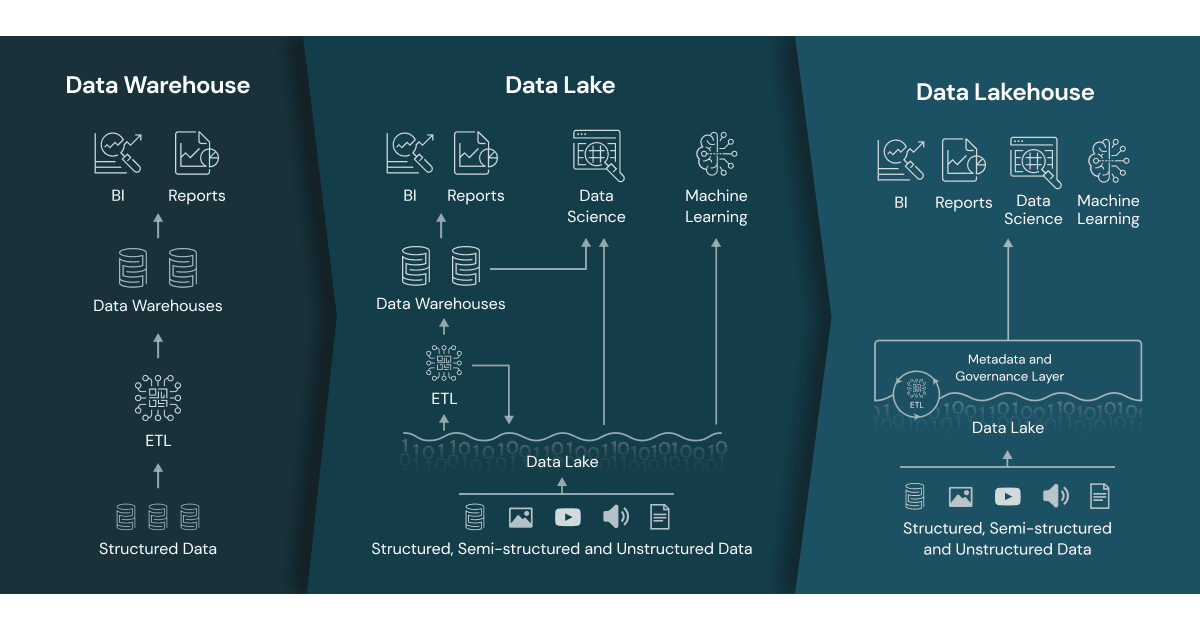
\includegraphics[width=\linewidth]{images/data-warehouse-data-lake-datalakehouse.png}
\caption{Data Warehouse vs Data Lake vs Data Lakehouse}\label{fig:data-warehouse-data-lake-datalakehouse}
\end{figure}

\section{Difference between Microservices Architecture and Monolithic Architecture}
\begin{enumerate}
\item[$\bullet$] \textbf{Monolithic:} A monolith is an application that is designed as a single, indivisible entity. All the application's functionalities are grouped together in a single code base, sharing the same resources, databases, and deployments. In a monolithic architecture, there is no clear separation of functionalities into independent services. Any modification or evolution of the application requires changes at a global level.
\item[$\bullet$] \textbf{Microservice:} A microservice is an architectural approach in which an application is built as a set of independent and autonomous services, each focusing on a specific function of the application. Each microservice is developed, deployed, and managed independently, allowing for easier scalability, flexibility, and maintenance. Microservices communicate with each other through well-defined interfaces, typically based on REST APIs or messaging.
\end{enumerate}

\subsection{Advantages and Disadvantages of Monolithic Architecture}
\textbf{Advantages:}
\begin{enumerate}
\item \textbf{Simplicity of initial development:} The monolithic approach allows for rapid development of an application by grouping all functionalities into a single code base. This simplifies dependency management and coordination of different parts of the application.
\item \textbf{Less operational complexity:} With a monolithic architecture, there are fewer components and services to manage, simplifying deployment, monitoring, and management operations. Everything is bundled within a single deployment, which can be easier to handle for operational teams.
\item \textbf{Faster internal communications:} In a monolithic architecture, communications between different parts of the application are faster as they typically occur through internal method calls. This can be beneficial in terms of performance and reduced latency.
\end{enumerate}

\textbf{Disadvantages:}
\begin{enumerate}
\item \textbf{Difficulty in scaling and maintaining:} With a monolithic architecture, scaling and updates can be more complex since every change needs to be made to the entire application. This can slow down the development process and pose risks of errors during deployments.
\item \textbf{Technological rigidity:} A monolithic architecture can result in technological rigidity as all parts of the application must use the same technologies and programming languages. This can limit the opportunities to adopt new technologies or independently evolve specific parts of the application.
\item \textbf{Difficulty in isolating issues:} In case of issues or bugs, it can be more challenging to isolate and resolve them in a monolithic architecture. Since all functionalities are grouped in a single code base, pinpointing the exact origin of the problem can be complex.
\item \textbf{Less flexibility in terms of scalability:} Monolithic architecture can pose challenges in terms of scalability. If a part of the application requires more resources to handle high load, adjusting that specific part without increasing the overall resources of the application can be difficult.
\end{enumerate}

\subsection{Advantages and Disadvantages of Microservices Architecture}
\textbf{Advantages:}
\begin{enumerate}
\item \textbf{Scalability and evolvability:} Microservices allow breaking down the application into several autonomous and independent services, facilitating horizontal scalability. Each microservice can be deployed, scaled, and updated independently, efficiently managing load variations and ensuring easy scalability according to business needs.
\item \textbf{Technological flexibility:} Microservices offer the ability to use different technologies and programming languages for each service. In our case, using Spring Boot allows us to leverage its rich ecosystem and advanced features for rapid application development. It also enables adopting specific technologies based on the needs of each microservice, promoting technological flexibility.
\item \textbf{Independence and autonomy:} Each microservice is designed to operate autonomously, allowing better isolation of functionalities and responsibilities. This facilitates maintenance, testing, and independent deployment of services, reducing the risks of impacting the entire system in case of changes or issues.
\item \textbf{Rapid development and deployment:} Microservices enable an agile development approach by emphasizing shorter development cycles. Teams can focus on specific features and develop them independently, accelerating the overall system development. Additionally, microservices can be continuously deployed through the use of automated deployment techniques, facilitating frequent and rapid updates.
\item \textbf{Ease of maintenance and debugging:} Due to their modular nature, microservices facilitate system maintenance and debugging. In case of problems or errors, it's easier to identify the specific service involved and resolve the issue without impacting the entire system.
\end{enumerate}

\textbf{Disadvantages:}
\begin{enumerate}
\item \textbf{Complexity in managing communications:} Microservices involve communication between different services, typically through REST APIs or messaging. Managing these communications can become complex, especially when numerous services are involved. Issues such as latency, data consistency, and error handling may arise.
\item \textbf{Increased initial development overhead:} Developing microservices requires additional effort to properly decompose functionalities, define interfaces, and set up appropriate infrastructure for service deployment and communication. This can increase the initial workload and require specific skills in distributed architecture.
\item \textbf{Managing data consistency:} With microservices, each service can have its own database or data storage. This can make managing data consistency more complex, particularly when simultaneous updates involving multiple services occur. Techniques such as distributed transactions or asynchronous events may be required to maintain data consistency.
\item \textbf{Deployment and management of multiple services:} With microservices, there is an increased number of services to deploy, manage, and monitor. This may require additional skills in automated deployments, container management, or cluster management. Monitoring the performance and behavior of each service can also become more complex.
\item \textbf{Infrastructure cost:} Microservices may require more complex infrastructure and additional resources to operate effectively. Each service needs to be deployed and run independently, which can result in increased costs related to computing resources and infrastructure management.
\end{enumerate}

\begin{figure}[H]
\centering
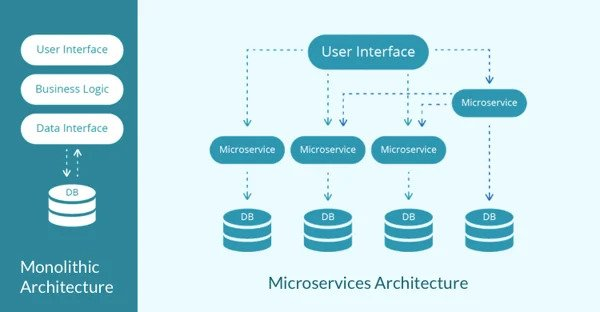
\includegraphics[width=0.6\linewidth]{images/monolithicvsmicroservice.jpg}
\caption{Monolithic Architecture vs Microservices Architecture}\label{fig:monolithicvsmicroservice}
\end{figure}

\section{Difference between Microfrontends Architecture and Monolithic Frontend Architecture}
\begin{enumerate}
\item[$\bullet$] \textbf{Monolithic Frontend:} A monolithic frontend architecture is an architectural approach where the frontend application is developed as a single entity, typically using a specific framework such as AngularJS. All the features, views, and user interface logic are grouped together in a single code base.
\item[$\bullet$] \textbf{Microfrontends:} Microfrontends are an architectural approach where a frontend application is divided into multiple independent micro-applications, each responsible for a specific part of the user interface. Each micro-application can be developed, deployed, and evolved independently, using different frameworks, languages, and technologies.
\end{enumerate}

\subsection{Advantages and Disadvantages of Monolithic Frontend Architecture}
\textbf{Advantages:}
\begin{enumerate}
\item \textbf{Simplicity of initial development:} The monolithic architecture with AngularJS provides a straightforward approach for the initial development of the frontend application. All the features are grouped together in a single code base, making it easier to coordinate and manage the development.
\item \textbf{Ease of communication between components:} In a monolithic architecture, AngularJS components can communicate with each other easily through the AngularJS directives and services system. This allows for quick and efficient communication between different parts of the application.
\item \textbf{Interoperability of features:} Since all the features are developed using AngularJS, it is easier to share features and modules between different parts of the application. This promotes code reuse and simplifies maintenance.
\end{enumerate}

\textbf{Disadvantages:}
\begin{enumerate}
\item \textbf{Difficulty in maintenance and scalability:} As the frontend application becomes more complex, maintaining and evolving the monolithic architecture with AngularJS can become challenging. Changes to one part of the application can have implications on the entire code base, making the development process slower and riskier.
\item \textbf{Performance limitations:} In a monolithic architecture, all the features are loaded together, which can lead to performance issues if the application becomes large. Loading times can be longer, and the application may be less responsive for the user.
\item \textbf{Limited flexibility:} The monolithic architecture with AngularJS can limit technological flexibility. Since all parts of the application are developed using AngularJS, it can be difficult to introduce new technologies or independently evolve specific parts of the application.
\end{enumerate}

\subsection{Advantages and Disadvantages of Microfrontends Architecture}
\textbf{Advantages:}
\begin{enumerate}
\item \textbf{Independence of development teams:} Each micro-application can be developed by a separate team, promoting greater autonomy and better collaboration among development teams. Each team can choose the technologies that best suit their needs.
\item \textbf{Scalability and ease of maintenance:} Microfrontends architecture allows for independent scaling and maintenance of different parts of the application. Changes to one micro-application do not impact others, making maintenance easier and enabling rapid deployment of new features.
\item \textbf{Technological flexibility:} Each micro-application can use the technology, framework, or programming language that best suits its specific domain. This allows for the introduction of new technologies and leveraging the benefits of the latest developments in software engineering.
\end{enumerate}

\textbf{Disadvantages:}
\begin{enumerate}
\item \textbf{Increased complexity:} Microfrontends architecture introduces some complexity in the development and deployment of the application. Managing interactions and communication between different micro-applications may require additional planning and coordination.
\item \textbf{Higher initial development cost:} Developing a microfrontends architecture may require a higher initial investment in terms of resources and time. Developing multiple separate micro-applications and setting up the necessary infrastructure can be more costly than developing a monolithic application.
\item \textbf{Network overhead:} Using microfrontends architecture can result in increased network overhead as each micro-application requires separate requests and resource loading. This can impact application performance and require efficient network management.
\end{enumerate}

\begin{figure}[H]
\centering
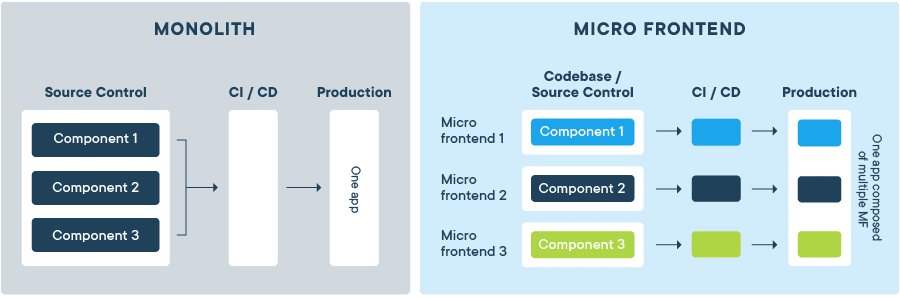
\includegraphics[width=\linewidth]{images/micro-frontend-vs-monolith-frontend.png}
\caption{Monolithic Frontend Architecture vs Microfrontends Architecture}\label{fig:monolithfrontendvsmicrofrontends}
\end{figure}

\section{Solution Approach}
\subsection{Data Part}
In the context of our solution, we have chosen to replace the existing exporter worker and MariaDB databases with the use of a data lakehouse architecture. A data lakehouse is a hybrid approach that combines the benefits of a data warehouse and a data lake, providing a more flexible and scalable solution for data management.

\subsection{Backend Part}
For the implementation of microservices, we have chosen to use Spring Boot, a popular Java framework for application development. By using Spring Boot, we can create standalone microservices that are independent of each other and can be developed, deployed, and scaled individually. Spring Boot also provides features such as data persistence management, security, and REST API creation, making it easier to develop microservices.

\subsection{Frontend Part}
For the implementation of microfrontends, we have primarily chosen to use React. The development team can benefit from the rich and mature React ecosystem, as well as its increasing popularity in the frontend development industry. However, it is also mentioned that Angular can be used later if needed, providing additional flexibility in the choice of technologies.

\section*{Conclusion}
When evaluating different data architectures for Izicap, it is important to understand the specific needs related to the management of bank files, transaction receipts, and aggregation operations.

A data warehouse could have been a viable option, offering structured and optimized data structures for analytical queries. However, the main drawback of a data warehouse lies in its static nature, which requires pre-modeling of data and rigid transformation before loading. This can pose challenges when integrating new file types or evolving aggregation requirements.

On the other hand, a data lake has advantages in terms of cost-effective storage and flexibility to integrate raw and unstructured data. However, maintaining data quality and governance can be more complex, and specific technical skills are required to effectively leverage data from the data lake.

Therefore, Delta Lake was favored due to its ability to meet Izicap's specific needs for managing bank files, transaction receipts, and aggregation operations. It provides the necessary flexibility and performance while maintaining data integrity, making it a solid choice for the company's data architecture.

By adopting a microservices-based approach, Izicap can improve the flexibility, scalability, and maintenance of its frontend application. This will enable the company to better meet the changing needs of its users, facilitate collaboration between development teams, and adopt innovative technologies to deliver an optimal user experience.

Microfrontends offer several advantages for Izicap. Firstly, the modularity inherent in microfrontends allows for the development, deployment, and maintenance of different parts of the user interface independently. This promotes collaboration between development teams and enables rapid and efficient evolution. Each micro-application can be developed using the framework and technologies that best suit its specific needs, providing essential technological flexibility for Izicap.

In contrast, the monolithic approach has limitations in terms of scalability and technological flexibility. Changes made to one part of the application can impact the entire system, making evolutions more complex and risky. Additionally, introducing new technologies or frameworks can be challenging in a monolithic architecture, limiting opportunities for innovation and modernization.